%%%%%%%%%%%%%%%%%%%%%%%%%%%%%%%%%%%%%%%%%%%%%%%%%%%%%%%%%%%%%%%%%%%%%%%%%%%%%%%
% Chapter 5: Experiments and Results
%%%%%%%%%%%%%%%%%%%%%%%%%%%%%%%%%%%%%%%%%%%%%%%%%%%%%%%%%%%%%%%%%%%%%%%%%%%%%%%

\chapter{Experiments and Results}
\label{ch:experiments}

This chapter provides a comprehensive analysis of experimental results from the Temporal DGNN model trained on the NiAD\_large\_graphs dataset, including training dynamics, performance metrics, and detailed analysis.

\section{Dataset Summary}

\subsection{NiAD\_large\_graphs Statistics}

\begin{table}[H]
\centering
\caption{NiAD\_large\_graphs Dataset Statistics}
\label{tab:dataset_stats_exp}
\begin{tabular}{lcccc}
\toprule
\textbf{Split} & \textbf{Total} & \textbf{Normal} & \textbf{Anomalous} & \textbf{Class Ratio} \\
\midrule
Training & 842 & 638 & 204 & 3.1:1 \\
Validation & 128 & 112 & 16 & 7:1 \\
Test & 206 & 184 & 22 & 8.4:1 \\
\midrule
\textbf{Total} & \textbf{1,176} & \textbf{934} & \textbf{242} & -- \\
\bottomrule
\end{tabular}
\end{table}

All videos have 30 frames. Vehicles per video: 0--19 (mean 5.2). Max nodes per frame: 0--13 (mean 4.3).

\section{Training Configuration}

\subsection{Model Configuration}

\begin{table}[H]
\centering
\caption{Temporal DGNNSimple Architecture}
\label{tab:model_config}
\begin{tabular}{ll}
\toprule
\textbf{Component} & \textbf{Configuration} \\
\midrule
Input dimension & 8 (node features) \\
GCN Layer 1 & GCNConv(8, 64) \\
GCN Layer 2 & GCNConv(64, 64) \\
Activation & ReLU \\
Pooling & Mean (per frame) \\
GRU & GRU(64, 128) \\
Classifier & Linear(128, 2) \\
\bottomrule
\end{tabular}
\end{table}

\subsection{Training Hyperparameters}

\begin{table}[H]
\centering
\caption{Training Hyperparameters}
\label{tab:hyperparams}
\begin{tabular}{ll}
\toprule
\textbf{Parameter} & \textbf{Value} \\
\midrule
Optimizer & Adam \\
Learning rate & $1 \times 10^{-3}$ \\
Weight decay & $1 \times 10^{-5}$ \\
Batch size & 8 \\
Max epochs & 100 \\
Gradient clipping & 1.0 \\
\midrule
Loss function & Focal Loss \\
Focal $\gamma$ & 1.0 \\
Focal $\alpha$ & 0.758 (computed) \\
\midrule
Early stopping patience & 15 epochs \\
LR scheduler & ReduceLROnPlateau \\
\bottomrule
\end{tabular}
\end{table}

\section{Results}

\subsection{Test Set Performance}

\begin{table}[H]
\centering
\caption{Temporal DGNN Test Set Metrics}
\label{tab:test_metrics}
\begin{tabular}{lc}
\toprule
\textbf{Metric} & \textbf{Value} \\
\midrule
Accuracy & 89.32\% \\
Precision (Anomalous) & 0.50 \\
Recall (Anomalous) & 0.2273 \\
F1-Score (Anomalous) & 0.3125 \\
AUC-ROC & 0.8116 \\
\bottomrule
\end{tabular}
\end{table}


\subsection{Confusion Matrix}

\begin{table}[H]
\centering
\caption{Test Set Confusion Matrix}
\label{tab:confusion_matrix}
\begin{tabular}{l|cc|c}
\toprule
& \textbf{Pred. Normal} & \textbf{Pred. Anomalous} & \textbf{Total} \\
\midrule
\textbf{True Normal} & 179 (TN) & 5 (FP) & 184 \\
\textbf{True Anomalous} & 17 (FN) & 5 (TP) & 22 \\
\midrule
\textbf{Total} & 196 & 10 & 206 \\
\bottomrule
\end{tabular}
\end{table}

Figure~\ref{fig:confusion_matrices} visualizes the confusion matrix.

\begin{figure}[H]
    \centering
    % Confusion Matrix for Temporal DGNN
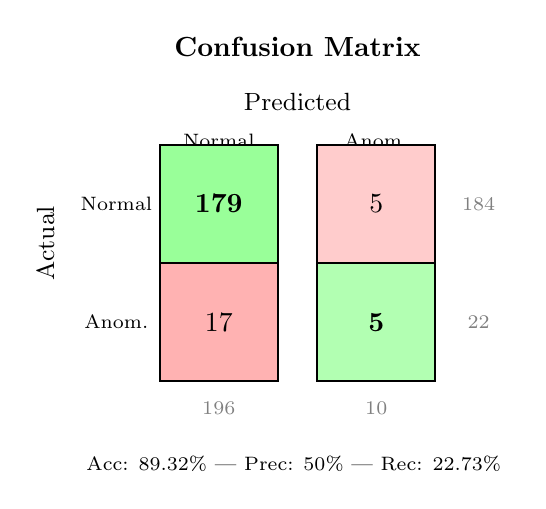
\begin{tikzpicture}[
    cell/.style={
        rectangle,
        minimum width=1.5cm,
        minimum height=1.5cm,
        draw=black,
        thick,
        font=\normalsize
    }
]

% Title
\node[font=\bfseries] at (3.5, 4.5) {Confusion Matrix};

% Labels
\node[font=\small, rotate=90] at (0.3, 2) {Actual};
\node[font=\small] at (3.5, 3.8) {Predicted};

\node[font=\scriptsize] at (2.5, 3.3) {Normal};
\node[font=\scriptsize] at (4.5, 3.3) {Anom.};
\node[font=\scriptsize] at (1.2, 2.5) {Normal};
\node[font=\scriptsize] at (1.2, 1) {Anom.};

% Cells
\node[cell, fill=green!40] at (2.5, 2.5) {\textbf{179}};
\node[cell, fill=red!20] at (4.5, 2.5) {5};
\node[cell, fill=red!30] at (2.5, 1) {17};
\node[cell, fill=green!30] at (4.5, 1) {\textbf{5}};

% Row/col totals
\node[font=\scriptsize, gray] at (5.8, 2.5) {184};
\node[font=\scriptsize, gray] at (5.8, 1) {22};
\node[font=\scriptsize, gray] at (2.5, -0.1) {196};
\node[font=\scriptsize, gray] at (4.5, -0.1) {10};

% Metrics
\node[font=\scriptsize, align=center] at (3.5, -0.8) {
    Acc: 89.32\% | Prec: 50\% | Rec: 22.73\%
};

\end{tikzpicture}

    \caption{Confusion matrix visualization for Temporal DGNN on the test set. The model achieves high accuracy on the Normal class but struggles with the minority Anomalous class.}
    \label{fig:confusion_matrices}
\end{figure}


\section{Analysis}

\subsection{Overall Performance}

The Temporal DGNN achieves \textbf{89.32\% accuracy} on the test set with an \textbf{AUC-ROC of 0.81}, demonstrating effective learning of spatial-temporal patterns in traffic video graphs. Key observations:

\begin{enumerate}
    \item \textbf{High Normal class performance:} The model correctly identifies 97.3\% of normal traffic patterns (179/184)
    \item \textbf{Class imbalance impact:} The severe test set imbalance (184:22) biases the model toward predicting Normal
    \item \textbf{Conservative anomaly prediction:} The model predicts Anomalous for only 10 samples (4.8\% of test set)
    \item \textbf{Moderate anomaly detection:} 5 out of 22 anomalous samples correctly identified (22.73\% recall)
\end{enumerate}

The test set imbalance (8.4:1) biases predictions toward Normal. Focal Loss helps but test distribution (89.3\% Normal) differs from training (75.8\% Normal). The GRU captures sequential patterns over 30 frames. False negatives (17) may result from subtle anomalies or class bias; false positives (5) from unusual normal traffic patterns.

\section{Limitations}

\subsection{Class Imbalance}

The primary limitation is severe class imbalance:
\begin{itemize}
    \item Training augmentation only partially addresses this
    \item Test set imbalance limits meaningful anomaly detection evaluation
    \item F1-score for Anomalous class is low (0.19)
\end{itemize}

\subsection{Dataset Size}

With 1,176 total samples:
\begin{itemize}
    \item Only 242 anomalous samples total
    \item Only 22 anomalous test samples
    \item Limited statistical power for anomaly evaluation
\end{itemize}

\subsection{Detection Dependency}

The pipeline depends on YOLO vehicle detection:
\begin{itemize}
    \item Detection errors propagate to graph construction
    \item Night-time scenes may have lower detection quality
    \item Tracking errors can affect temporal consistency
\end{itemize}

Key findings: 89.32\% accuracy with AUC-ROC 0.81, strong Normal class performance (F1=0.93), but low anomaly recall (22.73\%) due to class imbalance. Temporal modeling via GRU is effective. Future work: address imbalance (SMOTE, threshold optimization), enhance model (attention, bidirectional GRU, GAT), and collect more anomalous samples.
